\subsection{\Sh as a maximization problem} \label{GLOBALsec:formulas-sh}

In order to efficiently evaluate the seed heuristic, \cref{GLOBALeq:sh}, we rewrite it
from a minimization of match costs to a maximization of match scores. We first
define a few new concepts, and then rewrite the equation into form that will be
simpler to compute.

\paragraph{Score}
We define the \emph{score of a match} $m$ as $\matchscore(m):={r-\cost(m)}$.
This is always positive since match costs are defined to be strictly less than~$r$.
The \emph{score of a seed} $s$ is the maximal score of a match of $s$:
\begin{equation}
  \seedscore(s) := \begin{cases}
    \max_{m\in \matches_s} \matchscore(m) &\text{if $\matches_s \neq \emptyset$}, \\
    0 &\text{otherwise.}
  \end{cases}\label{GLOBALeq:seedscore}
\end{equation}
The \emph{score of a state} is the sum of the scores of the remaining seeds,
\begin{equation} \label{GLOBALeq:sh-score}
  \shscore\st ij := \sum_{s\in \seeds_{\geq i}} \seedscore(s).
\end{equation}

\paragraph{Potential} The \emph{potential} $\Pot\st ij$ is the value of the
heuristic when there are no matches, and is the maximal value the heuristic can
take in a given state:
\begin{equation} \label{GLOBALeq:potential}
  \Pot\st ij := r\cdot |\seeds_{\geq i}|.
\end{equation}

\paragraph{Objective}
\cref{GLOBALeq:sh} can now be rewritten in terms of potential
and score,
\begin{align}
  \hshM(u)
  &\stackrel{\text{\eqref{GLOBALeq:sh}}}= \sum_{s\in \seeds_{\geq i}}\left(r-\begin{cases}
    \max_{m\in \matches_s} r-\cost(m) &\text{if $\matches_s \neq \emptyset$}, \\
    0 &\text{otherwise}
  \end{cases}\right)\nonumber\\
  &= r\cdot |\seeds_{\geq i}| -
   \sum_{s\in \seeds_{\geq i}}\begin{cases}
    \max_{m\in \matches_s} \matchscore(m) &\text{if $\matches_s \neq \emptyset$}, \\
    0 &\text{otherwise}
  \end{cases}\nonumber\\
  &\stackrel{\text{\eqref{GLOBALeq:seedscore}}}{=} r\cdot |\seeds_{\geq i}| - \sum_{s\in \seeds_{\geq i}} \seedscore(s)
  \stackrel{\text{\eqref{GLOBALeq:sh-score},\eqref{GLOBALeq:potential}}}{=}\Pot(u) - \shscore(u).
  \label{GLOBALeq:sh-computation}
\end{align}
The potential $\Pot(u)$ of a state is simple to compute, and the score
$\shscore(u)$ can be computed by using \emph{layers}.

\paragraph{Layer}
Let \emph{layer} $\layer_\ell$ be the set of states $u$ with score
$\shscore(u) \geq \ell$.
Since $\shscore$ is non-increasing in $i$ and independent of $j$, and only
changes value at the start of seeds, $\layer_\ell$ is fully
determined by largest $i_\ell$ such that $\shscore\st {i_\ell}{{\cdot}} \geq \ell$.
The score $\shscore\st ij$ is then the largest $\ell$ such that $i_\ell \geq i$.


\subsection{\Csh as a maximization problem} \label{GLOBALsec:formulas-csh}

Similar to the \sh, we rewrite \cref{GLOBALeq:csh} into a maximization form that will be simpler to compute.

\paragraph{Chain score}
The \emph{score of a chain} is the sum of the scores of the matches in the chain.
Let $\chainscore(m)$ be the maximum score of a chain starting with match $m$. This
satisfies the recursion
\begin{equation}
\chainscore(m) := \matchscore(m) + \max_{m\preceq m' } \chainscore(m').
\label{GLOBALeq:chainscore}
\end{equation}
where this and the following maxima are taken as $0$ when they are over an empty
set. For the \csh, the score at a state is
\begin{equation} \label{GLOBALeq:csh-score}
  \cshscore(u) := \max_{u\preceq m} \chainscore(m).
\end{equation}

\paragraph{Objective} Similar to the \sh, the \csh is computed via the
following equality,
\begin{align}
  \hcshM(u)
  &\stackrel{\text{\eqref{GLOBALeq:csh}}}= \min_{\pi \in G \path u{v_t}}  \sum_{s\in \seeds_{\geq i}} \left(
    r -
    \begin{cases}
    \matchscore(\pi_s) &\text{if $\pi_s \in \matches_s$}, \\
    0 &\text{otherwise}
    \end{cases}
  \right)\nonumber\\
  &= r\cdot |\seeds_{\geq i}| -
    \max_{\pi \in G \path u{v_t}}  \sum_{s\in \seeds_{\geq i}}
    \begin{cases}
    \matchscore(\pi_s) &\text{if $\pi_s \in \matches_s$}, \\
    0 &\text{otherwise}
    \end{cases}
  \nonumber\\
  &= r\cdot |\seeds_{\geq i}| -
    \max_{u\preceq m_1\preceq \dots \preceq m_l}
      \big\{\matchscore(m_1) + \dots + \matchscore(m_l)\big\} \nonumber\\
  &\stackrel{\mathclap{\text{\eqref{GLOBALeq:potential},\eqref{GLOBALeq:csh-score}}}}=\ \Pot(u) - \cshscore(u).
  \label{GLOBALeq:csh-computation}
\end{align}

\begin{figure}[t]
  \centering
  \subfloat[Before]{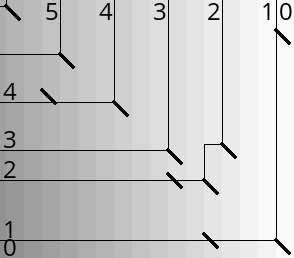
\includegraphics[width=0.4\linewidth]{imgs/fig3/start.png}\label{GLOBALfig:contours-start}}
  %\hfill
  \hspace{0.01\linewidth}
  \subfloat[After]{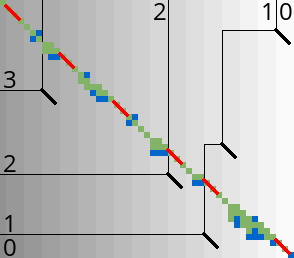
\includegraphics[width=0.4\linewidth]{imgs/fig3/end.png}\label{GLOBALfig:contours-end}}
  \caption[Execution of the chaining seed heuristic with pruning]{An example of
  the layers and contours used by the \csh before and after the \A execution
  with match pruning for $r{=}1$ and seed length $k{=}3$. Exact matches with
  ${\matchscore(m){=}1}$ are shown as black diagonal segments~(\blackmatch{}).
  \emph{Contours} are shown as horizontal and vertical black lines and indicate
  the bottom-right boundaries of \emph{layers} $\layer_\ell$ consisting of the
  states above/left of the contour marked with $\ell$. States $u$ between two
  contours have the same maximal number of matches $\cshscore(u)$ on a chain to
  the end. The value of the heuristic is shown in the background, from white
  ($h{=}0$) to darker grey.  Expanded states are shown in
  green~(\greensquare{}), open states in blue~(\bluesquare{}), and pruned
  matches in red~(\redmatch{}). Note that pruning matches during the \A
  execution shifts the contours and changes the layers. This figure is produced
  by Ragnar~Groot Koerkamp and Mykola~Akulov.}
  \label{GLOBALfig:contours}
\end{figure}


\paragraph{Contours}
Like fore the \sh, we define layer $\layer_\ell$ as those states $u$ with score
$\cshscore(u)$ \emph{at least} $\ell$.
The $\ell$th \emph{contour} is
the bottom-right boundary of $\layer_\ell$ (see~\cref{GLOBALfig:contours}). A state
$u\in \layer_\ell$ is \emph{dominant} when there is no state $v\in \layer_\ell$ with
$v\neq u$ and $u\preceq v$. Both $\layer_\ell$ and the corresponding contour are completely
determined by the matches starting in the dominant states. The following lemma
makes this precise:
\begin{lem}\label{GLOBALlem:contour}
  For $\ell>0$
  the matches $m$ with $\ell \leq \chainscore(m) < \ell+r$ fully determine layer $\layer_\ell$:
  \begin{equation}
    \layer_\ell = \{u \mid \exists m\in \matches : u \preceq m \text{ \emph{and} } \ell \leq \chainscore(m) < \ell+r\}.
  \end{equation}
\end{lem}
\begin{proof}
  It follows directly from \cref{GLOBALeq:csh-score} that
  $\layer_\ell = \{u\mid \exists m\in \matches : u\preceq m \text{ and } \chainscore(m) \geq \ell\}$.
  Suppose that $m$ has score $\chainscore(m)\geq \ell+r$. By definition,
  $\matchscore(m) \leq r$, so by \cref{GLOBALeq:chainscore} there must be a match $m\preceq m'$ with
  $\chainscore(m') = \chainscore(m) - \matchscore(m) \geq (\ell+r)-r=\ell$. This implies that $u\preceq m\preceq m'$,
  which allows $m$, and hence any match with $\chainscore(m) \geq \ell+r$, to be omitted from consideration.
\end{proof}

We will use this lemma to efficiently find the largest $\ell$ such that layer
$\layer_\ell$ contains a state $u$, which gives $\cshscore(u)$.

Note that the formulas for the \csh become equivalent to those for the \sh when
the partial order ${\st ij\preceq\st{i'}{j'}}$ is redefined to mean $i \leq i'$,
ignoring the $j$-coordinate.
